\documentclass[11pt,a4paper]{article}

\usepackage[utf8]{inputenc}
\usepackage[T1]{fontenc}
\usepackage[spanish]{babel}
\usepackage{geometry}
\usepackage{graphicx}
\usepackage{array}
\usepackage{tabularx}
\usepackage{xcolor}
\usepackage{fancyhdr}
\usepackage{titlesec}
\usepackage{helvet}
\usepackage{ragged2e}
\usepackage{enumitem}
\usepackage{amsmath}
\usepackage{booktabs}
\usepackage{hyperref}

\renewcommand{\familydefault}{\sfdefault}
% babel-spanish names tables "Cuadro"; the report uses the Latin-American "Tabla".
\addto\captionsspanish{\renewcommand{\tablename}{Tabla}}
\graphicspath{{dist/}{./}}

\geometry{
  a4paper,
  left=3.0cm,
  right=3.0cm,
  top=2.35cm,
  bottom=2.35cm,
  headheight=1.9cm,
  headsep=0.45cm
}

\hypersetup{
  colorlinks=true,
  linkcolor=black,
  citecolor=black,
  urlcolor=blue
}

\setlength{\parindent}{0pt}
\setlength{\parskip}{0.22em}
\setlength{\tabcolsep}{6pt}
\renewcommand{\arraystretch}{1.08}

% Long unbreakable tokens (file names, inline math) otherwise overflow the margin.
\tolerance=1500
\emergencystretch=1.5em
\hyphenpenalty=200

\pagestyle{fancy}
\fancyhf{}
\fancyhead[L]{
\includegraphics[height=1.35cm]{reporte_tecnico_overleaf_logo.png}}
\fancyhead[R]{\vspace{0.1cm}\small FEIRNNR --- Carrera de Computaci\'on}
\renewcommand{\headrulewidth}{0.5pt}
\renewcommand{\footrulewidth}{0pt}
\makeatletter
\renewcommand{\headrule}{%
  {\color{gray!65}\hrule width\headwidth height\headrulewidth \vskip-\headrulewidth}%
}
\makeatother

\titleformat{\section}
  {\bfseries\fontsize{15}{17}\selectfont}
  {\thesection.}{0.8em}{}
\titlespacing*{\section}{0pt}{0.7ex}{0.2ex}

\titleformat{\subsection}
  {\bfseries\fontsize{12}{14}\selectfont}
  {\thesubsection}{0.7em}{}
\titlespacing*{\subsection}{0pt}{0.6ex}{0.15ex}

\newcolumntype{L}[1]{>{\RaggedRight\arraybackslash}p{#1}}
\newcolumntype{Y}{>{\RaggedRight\arraybackslash}X}
\newcolumntype{C}[1]{>{\centering\arraybackslash}p{#1}}

\begin{document}
\thispagestyle{fancy}

\vspace*{0.15cm}

\begin{center}
{\bfseries\fontsize{23}{26}\selectfont
Reporte T\'ecnico de Actividades\\
Pr\'actico-Experimentales Nro. 002\par}
\end{center}

\section{Datos de Identificaci\'on del Estudiante y la Pr\'actica}

\noindent
\begin{tabularx}{\textwidth}{|L{0.43\textwidth}|Y|}
\hline
\textbf{Nombre del estudiante} & Jaime Alejandro Land\'azuri Rom\'an \\ \hline
\textbf{Asignatura} & Simulaci\'on \\ \hline
\textbf{Ciclo} & 5 A \\ \hline
\textbf{Unidad} & U1: Introducci\'on a la Simulaci\'on \\ \hline
\textbf{Resultado de aprendizaje de la unidad} & R1. Aplica an\'alisis estad\'isticos de los
datos de la Simulaci\'on para mejorar la calidad de los resultados, bajo los principios de
solidaridad, transparencia, responsabilidad y honestidad. \\ \hline
\textbf{Pr\'actica Nro.} & 002 \\ \hline
\textbf{T\'itulo de la Pr\'actica} & Comparaci\'on de modelos determin\'isticos,
estoc\'asticos, discretos y continuos \\ \hline
\textbf{Nombre del Docente} & Jos\'e O. Guam\'an Q. \\ \hline
\textbf{Fecha} & 08 de Octubre de 2026 / 09 de Octubre de 2026 \\ \hline
\textbf{Horario} & Jueves 10h30 -- 11h30 / Viernes 07h30 -- 09h30 \\ \hline
\textbf{Lugar} & Aula \\ \hline
\textbf{Tiempo planificado en el S\'ilabo} & 3 horas \\ \hline
\end{tabularx}

\section{Objetivo(s) de la Pr\'actica}

Diferenciar los principales paradigmas de simulaci\'on mediante la construcci\'on de modelos
computacionales.

\begin{enumerate}[leftmargin=*]
  \item Implementar un modelo determin\'istico y uno estoc\'astico.
  \item Comparar modelos discretos y continuos.
  \item Analizar el efecto de la aleatoriedad sobre los resultados.
\end{enumerate}

\section{Materiales y Reactivos}

\begin{itemize}[leftmargin=*]
  \item Computadora con m\'inimo 4\,GB de RAM y procesador de doble n\'ucleo o superior.
  \item Sistema operativo Linux o macOS.
  \item Python 3.x, NumPy y Matplotlib.
  \item Visual Studio Code, PyCharm o Jupyter Notebook.
  \item Conexi\'on a Internet para instalar las herramientas.
\end{itemize}

\section{Fundamento Te\'orico}

Un modelo de simulaci\'on representa el comportamiento de un sistema mediante variables,
par\'ametros, ecuaciones y reglas \cite{lawkelton2015}. El sistema de estudio de esta
pr\'actica es el \textbf{crecimiento poblacional}, descrito por la ecuaci\'on diferencial
log\'istica en su r\'egimen inicial, donde la poblaci\'on crece sin l\'imite de recursos:

\begin{equation}
\frac{dP}{dt} = r\,P
\label{eq:edo}
\end{equation}

cuya soluci\'on exacta es el crecimiento exponencial propuesto originalmente por Malthus
\cite{malthus1798}:

\begin{equation}
P(t) = P_0\,e^{r t}
\label{eq:exponencial}
\end{equation}

donde $P_0$ es la poblaci\'on inicial, $P(t)$ la poblaci\'on en el tiempo $t$ y $r$ la tasa
de crecimiento. La ecuaci\'on \eqref{eq:edo} es \emph{lineal y aut\'onoma}: como el
incremento es proporcional a la poblaci\'on existente, genera realimentaci\'on positiva y
un comportamiento exponencial creciente si $r>0$, constante si $r=0$ y decreciente si
$r<0$ \cite{strogatz2015}.

A partir de este mismo sistema se construyen los cuatro paradigmas que se comparan en la
pr\'actica \cite{diaposSemana2}.

\subsection{Modelo determin\'istico}

Se utiliza directamente la soluci\'on anal\'itica de la ecuaci\'on \eqref{eq:exponencial}.
No se emplea aleatoriedad: el resultado queda un\'ivocamente determinado por $P_0$, $r$ y
$t$.

\subsection{Modelo discreto}

La poblaci\'on cambia en intervalos de tiempo definidos. El incremento se calcula sobre la
poblaci\'on actual y se acumula, lo que produce la sucesi\'on geom\'etrica:

\begin{equation}
P_{k+1} = P_k + r\,P_k = (1+r)\,P_k
\qquad\Longrightarrow\qquad
P_k = P_0\,(1+r)^{k}
\label{eq:discreto}
\end{equation}

El factor $(1+r)$ es la \emph{raz\'on de crecimiento por per\'iodo}.

\subsection{Modelo estoc\'astico}

Se incorpora una variable aleatoria aditiva $\varepsilon_k$ con distribuci\'on normal de
media cero y desviaci\'on est\'andar $\sigma$, que representa el nivel de variabilidad o
incertidumbre del sistema \cite{ross2014}:

\begin{equation}
P_{k+1} = P_k + r\,P_k + \varepsilon_k,
\qquad \varepsilon_k \sim \mathcal{N}\!\left(0,\sigma^{2}\right)
\label{eq:estocastico}
\end{equation}

Como una poblaci\'on negativa carece de sentido f\'isico, se aplica un truncamiento
inferior:

\begin{equation}
P_{k+1} \leftarrow \max\!\left(P_{k+1},\,0\right)
\label{eq:truncamiento}
\end{equation}

Este truncamiento es no lineal y provoca que, cuando $\sigma$ es grande, la media de las
trayectorias quede ligeramente por debajo de la trayectoria determinista.

\subsection{Modelo continuo mediante Euler}

El modelo continuo mantiene la ecuaci\'on diferencial \eqref{eq:edo}, pero se resuelve por
aproximaci\'on num\'erica de Euler con paso $\Delta t$ \cite{burden2011}:

\begin{equation}
P_{k+1} = P_k + \Delta t\,\left(r\,P_k\right) = \left(1 + r\,\Delta t\right)P_k
\label{eq:euler}
\end{equation}

El m\'etodo de Euler es de \textbf{primer orden}: su error de truncamiento local es
$O(\Delta t^{2})$ y el error global $O(\Delta t)$, de modo que $P_k$ converge a
$P(t) = P_0e^{rt}$ cuando $\Delta t \to 0$. N\'otese que, si $\Delta t = 1$, la ecuaci\'on
\eqref{eq:euler} coincide exactamente con el modelo discreto \eqref{eq:discreto}: ambos
paradigmas son el mismo c\'alculo visto con distinta resoluci\'on temporal.

\section{Procedimiento / Metodolog\'ia Ejecutada}

El desarrollo sigui\'o las cinco etapas indicadas a continuaci\'on, conforme a la gu\'ia de
actividades pr\'actico-experimentales Nro. 002 \cite{guaman2026ape2}.

\subsection{Preparaci\'on del entorno}

Se cre\'o un entorno virtual de Python y se instalaron las dependencias declaradas en
\texttt{requirements.txt} (\texttt{numpy}, \texttt{matplotlib} y \texttt{pandas}). La gu\'ia
menciona adem\'as \texttt{scipy} y \texttt{pynetlogo}; no fueron necesarias porque el
pseudocódigo es \'integramente Python y las gr\'aficas se generan con Matplotlib, por lo
que no se declararon dependencias sin uso.

\subsection{Serie de entrada}

Se utiliz\'o la serie de poblaci\'on observada indicada por la gu\'ia, que act\'ua como
condici\'on inicial, horizonte de simulaci\'on y referencia de validaci\'on
(ecuaci\'on \eqref{eq:entrada}):

\begin{equation}
\texttt{datos} = \left[1000,\;1100,\;1250,\;1400,\;1600,\;1850,\;2100\right]
\label{eq:entrada}
\end{equation}

De aqu\'i se obtienen $P_0 = 1000$ y $6$ per\'iodos de simulaci\'on.

\subsection{Implementaci\'on de los cuatro modelos}

Se implementaron las ecuaciones \eqref{eq:exponencial}, \eqref{eq:discreto},
\eqref{eq:estocastico}--\eqref{eq:truncamiento} y \eqref{eq:euler} siguiendo el
pseudoc\'odigo de la gu\'ia. Cada modelo devuelve un valor por per\'iodo, de manera que las
cuatro series se comparan sobre la misma malla entera $k = 0,\dots,6$. Los par\'ametros de
la corrida base se presentan en la tabla \ref{tab:parametros}.

\begin{table}[htbp]
\centering
\caption{Par\'ametros de la corrida base.}
\label{tab:parametros}
\small
\begin{tabular}{llc}
\toprule
\textbf{Par\'ametro} & \textbf{Significado} & \textbf{Valor} \\
\midrule
$P_0$    & Poblaci\'on inicial            & $1000$ \\
$r$      & Tasa de crecimiento            & $0{,}08$ \\
$\sigma$ & Nivel de ruido del modelo estoc\'astico & $40$ \\
$\Delta t$ & Paso de integraci\'on de Euler & $0{,}1$ \\
Per\'iodos & Horizonte de simulaci\'on    & $6$ \\
Semilla  & Semilla del generador aleatorio & $42$ \\
\bottomrule
\end{tabular}
\end{table}

La semilla se fij\'o en $42$ con el fin de que el modelo estoc\'astico sea
\emph{reproducible}: dos ejecuciones con los mismos par\'ametros producen exactamente los
mismos valores, requisito indispensable para que los resultados de este reporte sean
verificables.

\subsection{Estimaci\'on de la tasa $r$ a partir de los datos}

Dado que la identificaci\'on de la influencia de $r$ es un resultado esperado de la
pr\'actica, se estim\'o su valor desde la propia serie observada con dos estimadores:

\begin{itemize}[leftmargin=*]
  \item \textbf{Tasa discreta:} la media aritm\'etica de las razones
        per\'iodo a per\'iodo menos uno,
        $\hat{r} = \overline{\left(P_{k+1}/P_{k}\right)} - 1$.
  \item \textbf{Tasa continua:} la pendiente de la regresi\'on lineal de $\ln P$ contra
        $k$, que corresponde al exponente de la soluci\'on exacta
        \eqref{eq:exponencial}.
\end{itemize}

Ambos estimadores son distintos por construcci\'on y se relacionan mediante
$r_{\text{continuo}} = \ln\!\left(1 + r_{\text{discreto}}\right)$.

\subsection{Generaci\'on de resultados}

Se ejecut\'o el programa con la corrida base y con la tasa estimada, y se generaron las
gr\'aficas comparativas, los gr\'aficos de sensibilidad de $r$, $\sigma$ y $\Delta t$, y el
archivo \texttt{dist/\allowbreak resultados.csv}. La corrida con $r<0$ se us\'o para verificar el
r\'egimen de decrecimiento.

\section{Resultados}

\subsection{Corrida base con $r = 0{,}08$}

La tabla \ref{tab:base} presenta los valores de los cuatro modelos frente a la serie
observada, y la figura \ref{fig:comparacion} su representaci\'on gr\'afica.

\begin{table}[htbp]
\centering
\caption{Resultados de la corrida base ($r = 0{,}08$, $\sigma = 40$, $\Delta t = 0{,}1$, semilla $42$). Las columnas son los per\'iodos $0$ a $6$.}
\label{tab:base}
\small
\setlength{\tabcolsep}{4pt}
\begin{tabular}{L{3.2cm} C{1.3cm} C{1.3cm} C{1.3cm} C{1.3cm} C{1.3cm} C{1.3cm} C{1.3cm}}
\toprule
\textbf{Serie} & \textbf{0} & \textbf{1} & \textbf{2} & \textbf{3} & \textbf{4} & \textbf{5} & \textbf{6} \\
\midrule
Observado        & 1000{,}00 & 1100{,}00 & 1250{,}00 & 1400{,}00 & 1600{,}00 & 1850{,}00 & 2100{,}00 \\
Determin\'istico & 1000{,}00 & 1083{,}29 & 1173{,}51 & 1271{,}25 & 1377{,}13 & 1491{,}82 & 1616{,}07 \\
Discreto         & 1000{,}00 & 1080{,}00 & 1166{,}40 & 1259{,}71 & 1360{,}49 & 1469{,}33 & 1586{,}87 \\
Estoc\'astico    & 1000{,}00 & 1092{,}19 & 1137{,}96 & 1259{,}02 & 1397{,}36 & 1431{,}11 & 1493{,}51 \\
Euler (continuo) & 1000{,}00 & 1082{,}94 & 1172{,}76 & 1270{,}04 & 1375{,}38 & 1489{,}45 & 1612{,}99 \\
\bottomrule
\end{tabular}
\end{table}

\begin{figure}[htbp]
\centering
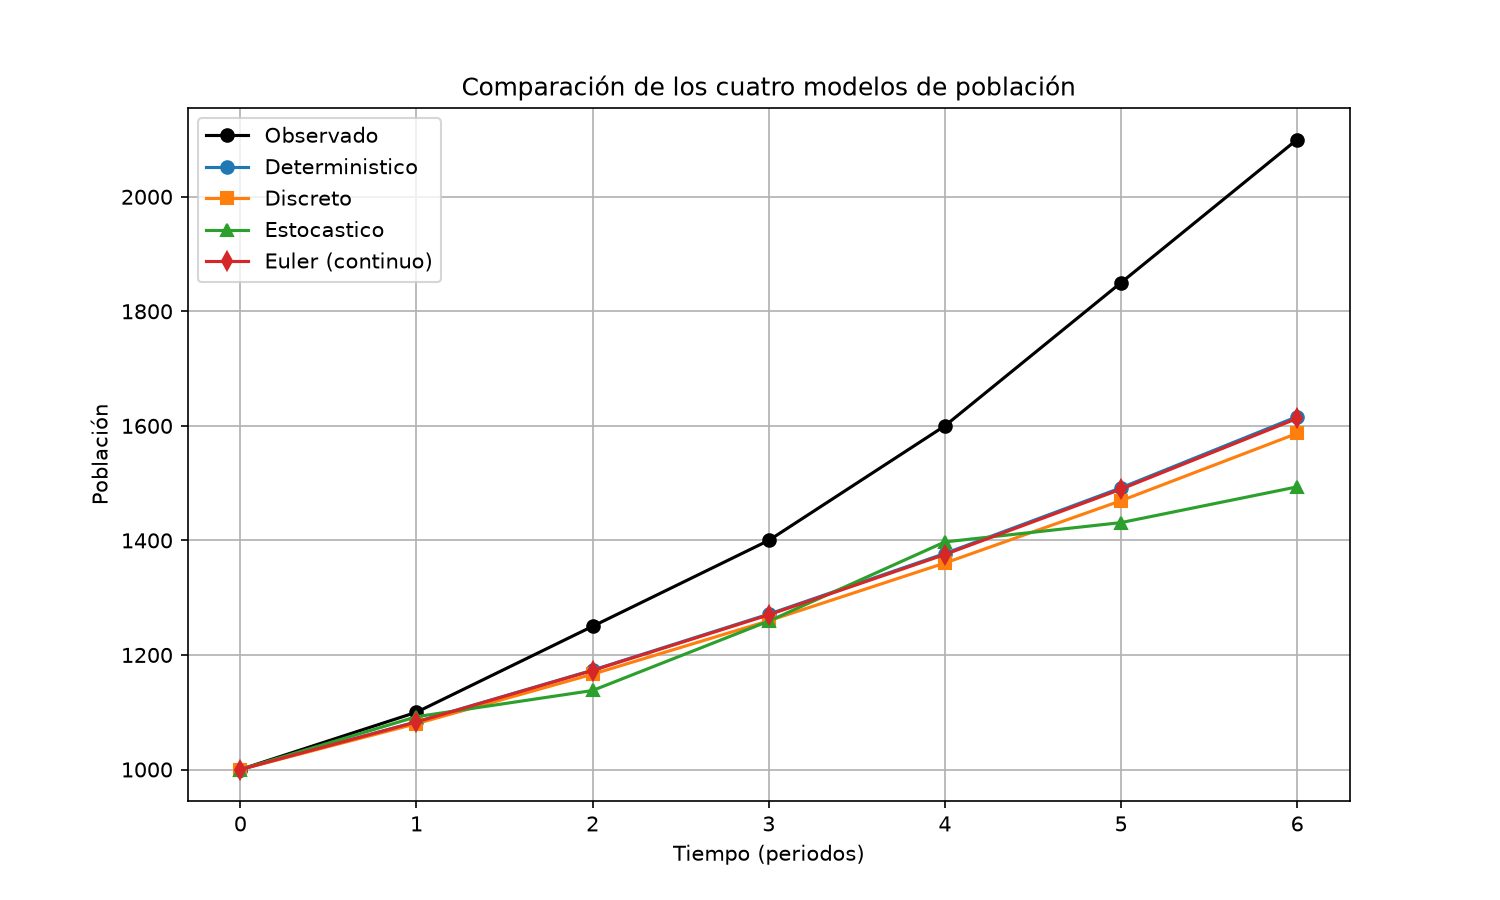
\includegraphics[width=0.92\textwidth]{comparacion_modelos.png}
\caption{Comparaci\'on de los cuatro modelos frente a la serie observada con $r = 0{,}08$.}
\label{fig:comparacion}
\end{figure}

Con $r = 0{,}08$ los cuatro modelos \textbf{subestiman} la poblaci\'on observada, porque la
serie real crece un 13{,}18\% por per\'iodo y no un 8\%. El error cuadr\'atico medio
(RMSE) de cada modelo frente a los datos se resume en la tabla \ref{tab:rmse}.

\begin{table}[htbp]
\centering
\caption{Error cuadr\'atico medio (RMSE) de cada modelo frente a la serie observada.}
\label{tab:rmse}
\small
\begin{tabular}{lcc}
\toprule
\textbf{Modelo} & \textbf{RMSE con $r = 0{,}08$} & \textbf{RMSE con $r = 0{,}1318$} \\
\midrule
Determin\'istico & 249{,}24 & 73{,}81 \\
Discreto         & 265{,}29 & \textbf{29{,}61} \\
Estoc\'astico    & 296{,}85 & 53{,}02 \\
Euler (continuo) & 250{,}93 & 68{,}22 \\
\bottomrule
\end{tabular}
\end{table}

\subsection{Estimaci\'on de la tasa $r$}

La tabla \ref{tab:estimacion} muestra los valores estimados a partir de la serie
observada. La tasa discreta es $0{,}1318$ y la continua $0{,}1254$; la diferencia es la
esperada, ya que $\ln(1{,}1318) = 0{,}1238$ es muy cercano al valor continuo obtenido por
m\'inimos cuadrados. La figura \ref{fig:ajuste} evidencia el ajuste.

\begin{table}[htbp]
\centering
\caption{Tasa de crecimiento estimada desde la serie observada.}
\label{tab:estimacion}
\small
\begin{tabular}{lc}
\toprule
\textbf{Estimador} & \textbf{Valor} \\
\midrule
Tasa discreta (media de las razones $-\,1$)   & $0{,}1318$ \\
Tasa continua (pendiente de $\ln P$ vs. $k$)  & $0{,}1254$ \\
Factor de crecimiento medio                   & $1{,}1318$ \\
\bottomrule
\end{tabular}
\end{table}

\begin{figure}[htbp]
\centering
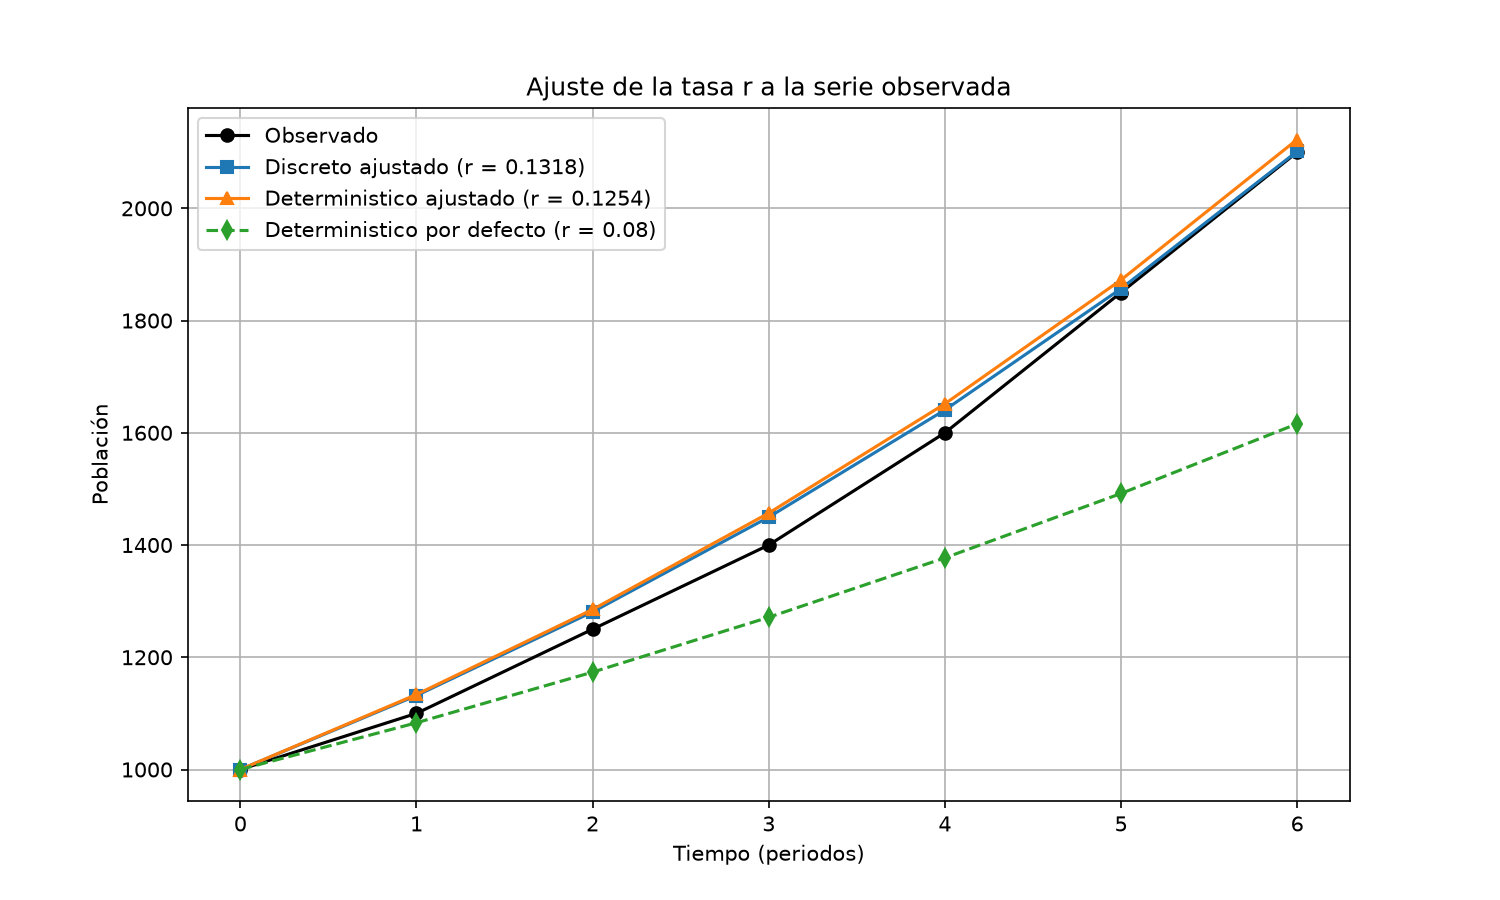
\includegraphics[width=0.92\textwidth]{ajuste_r.png}
\caption{Ajuste de la tasa estimada a la serie observada. La l\'inea discontinua es el
modelo determin\'istico con el valor de la gu\'ia ($r = 0{,}08$).}
\label{fig:ajuste}
\end{figure}

\subsection{Corrida con la tasa estimada}

Al reemplazar $r$ por la tasa estimada, el modelo discreto pasa a reproducir la serie
observada con un RMSE de $29{,}61$, frente a $265{,}29$ de la corrida base: una reducci\'on
de casi el 90\% del error (tabla \ref{tab:ajustada}).

\begin{table}[htbp]
\centering
\caption{Resultados con la tasa estimada ($r = 0{,}1318$). Las columnas son los per\'iodos $0$ a $6$.}
\label{tab:ajustada}
\small
\setlength{\tabcolsep}{4pt}
\begin{tabular}{L{3.2cm} C{1.3cm} C{1.3cm} C{1.3cm} C{1.3cm} C{1.3cm} C{1.3cm} C{1.3cm}}
\toprule
\textbf{Serie} & \textbf{0} & \textbf{1} & \textbf{2} & \textbf{3} & \textbf{4} & \textbf{5} & \textbf{6} \\
\midrule
Observado        & 1000{,}00 & 1100{,}00 & 1250{,}00 & 1400{,}00 & 1600{,}00 & 1850{,}00 & 2100{,}00 \\
Determin\'istico & 1000{,}00 & 1140{,}84 & 1301{,}52 & 1484{,}83 & 1693{,}96 & 1932{,}55 & 2204{,}73 \\
Discreto         & 1000{,}00 & 1131{,}77 & 1280{,}90 & 1449{,}68 & 1640{,}70 & 1856{,}89 & 2101{,}57 \\
Estoc\'astico    & 1000{,}00 & 1143{,}96 & 1253{,}09 & 1448{,}23 & 1676{,}68 & 1819{,}57 & 2007{,}25 \\
Euler (continuo) & 1000{,}00 & 1139{,}86 & 1299{,}29 & 1481{,}01 & 1688{,}14 & 1924{,}25 & 2193{,}38 \\
\bottomrule
\end{tabular}
\end{table}

\subsection{Sensibilidad a la tasa $r$}

La figura \ref{fig:influencia} muestra el efecto de variar $r$ en el modelo
determin\'istico, y la figura \ref{fig:crecdec} contrasta expl\'icitamente los reg\'imenes
de crecimiento ($r = +0{,}12$) y decrecimiento ($r = -0{,}12$).

\begin{figure}[htbp]
\centering
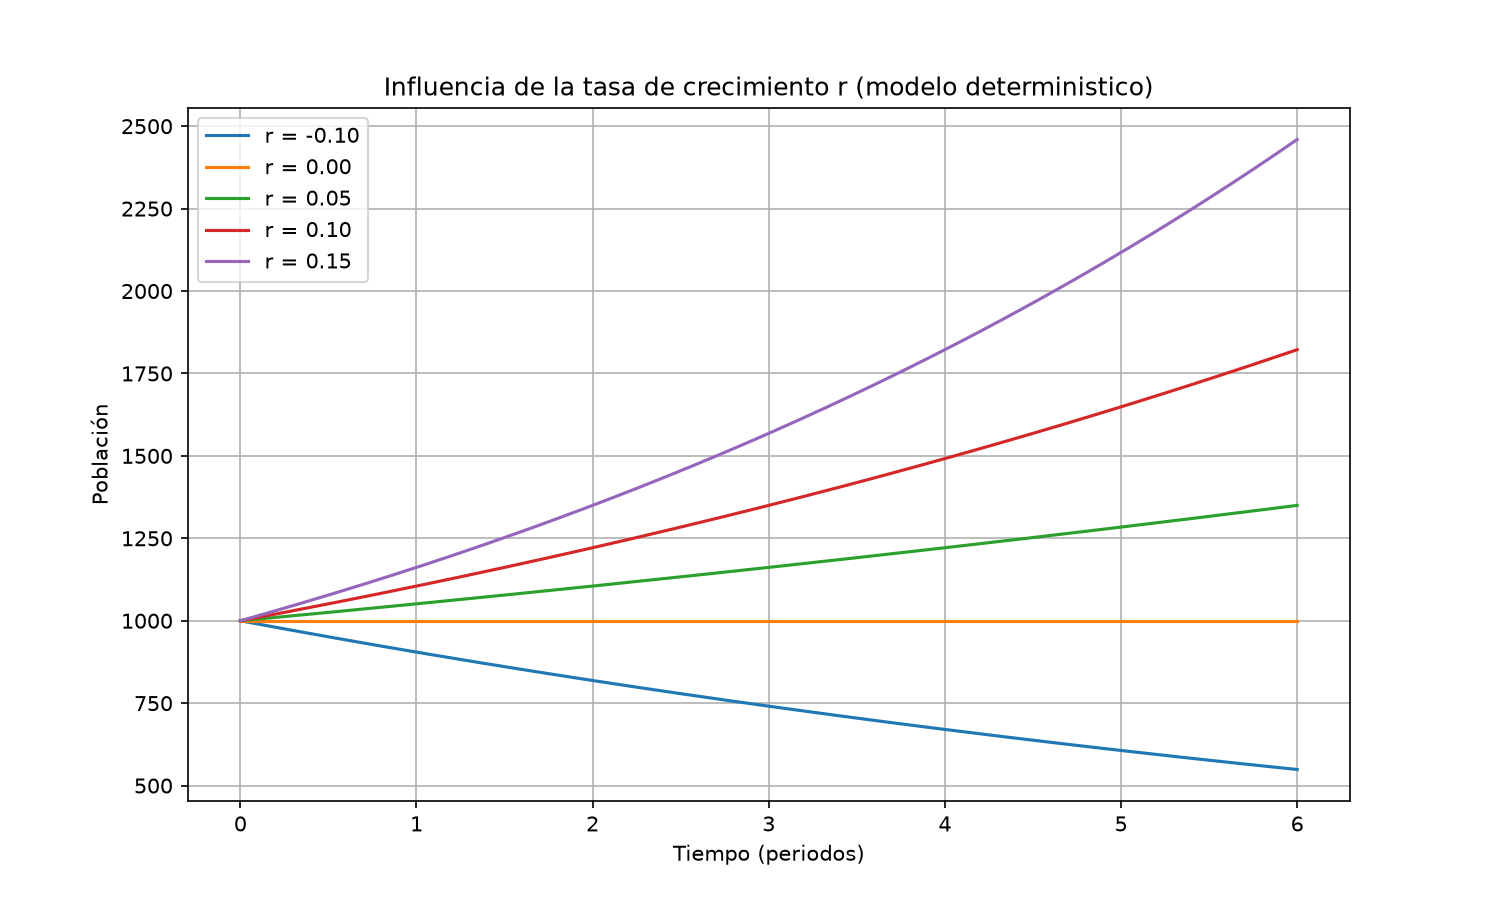
\includegraphics[width=0.92\textwidth]{influencia_r.png}
\caption{Influencia de la tasa de crecimiento $r$ en el modelo determin\'istico.}
\label{fig:influencia}
\end{figure}

\begin{figure}[htbp]
\centering
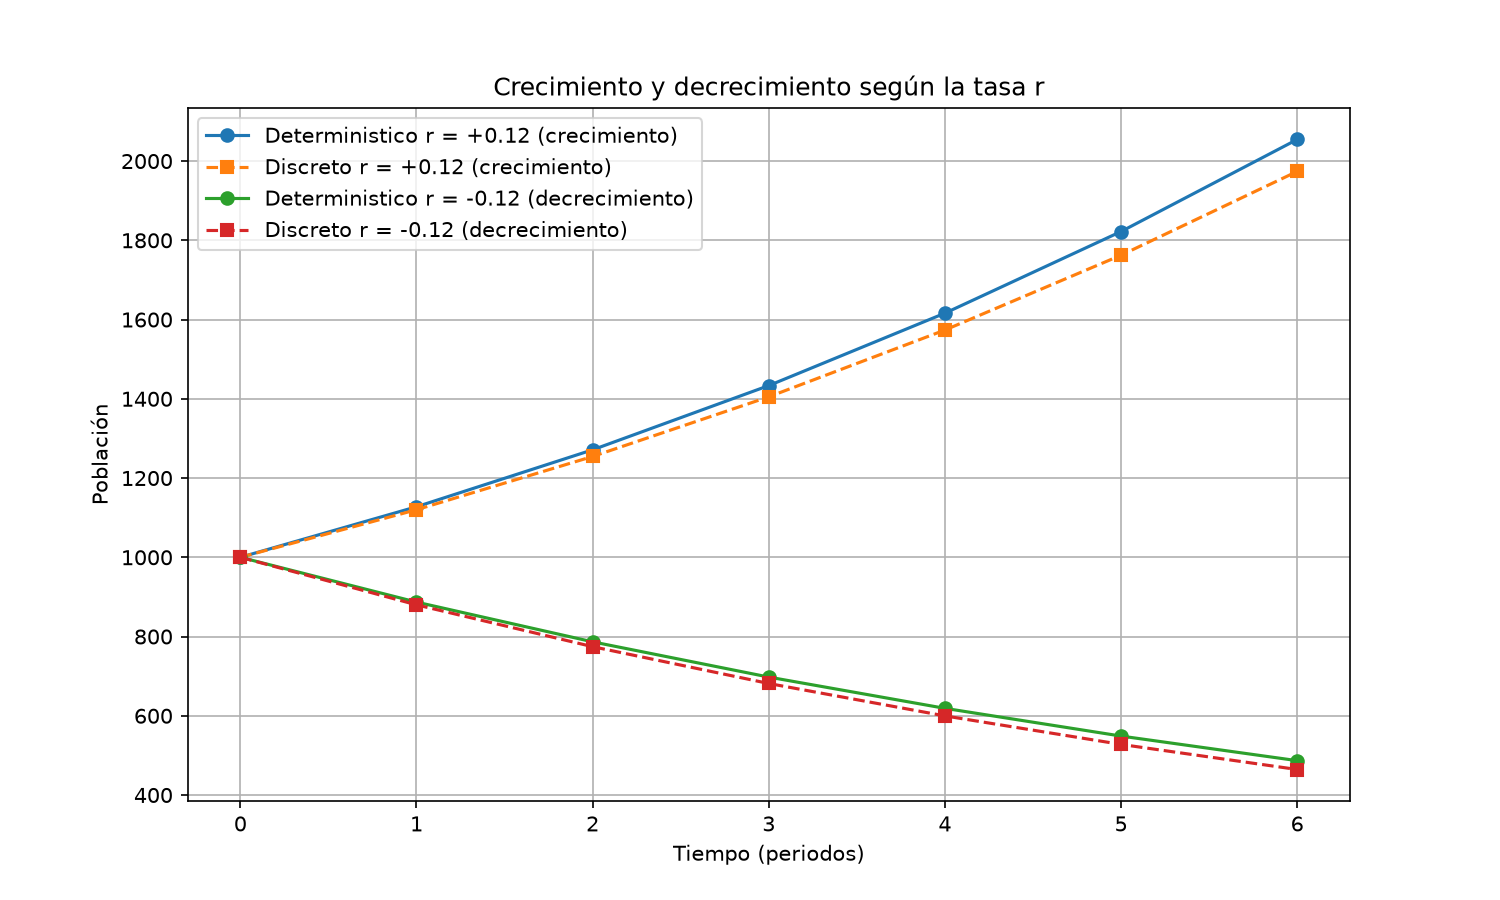
\includegraphics[width=0.92\textwidth]{crecimiento_decrecimiento.png}
\caption{Crecimiento ($r = +0{,}12$) y decrecimiento ($r = -0{,}12$) en los modelos
determin\'istico y discreto.}
\label{fig:crecdec}
\end{figure}

\subsection{Efecto de la aleatoriedad ($\sigma$)}

La figura \ref{fig:sigma} resume $30$ corridas independientes por cada nivel de ruido,
mostrando la media y la banda de $\pm 1$ desviaci\'on est\'andar.

\begin{figure}[htbp]
\centering
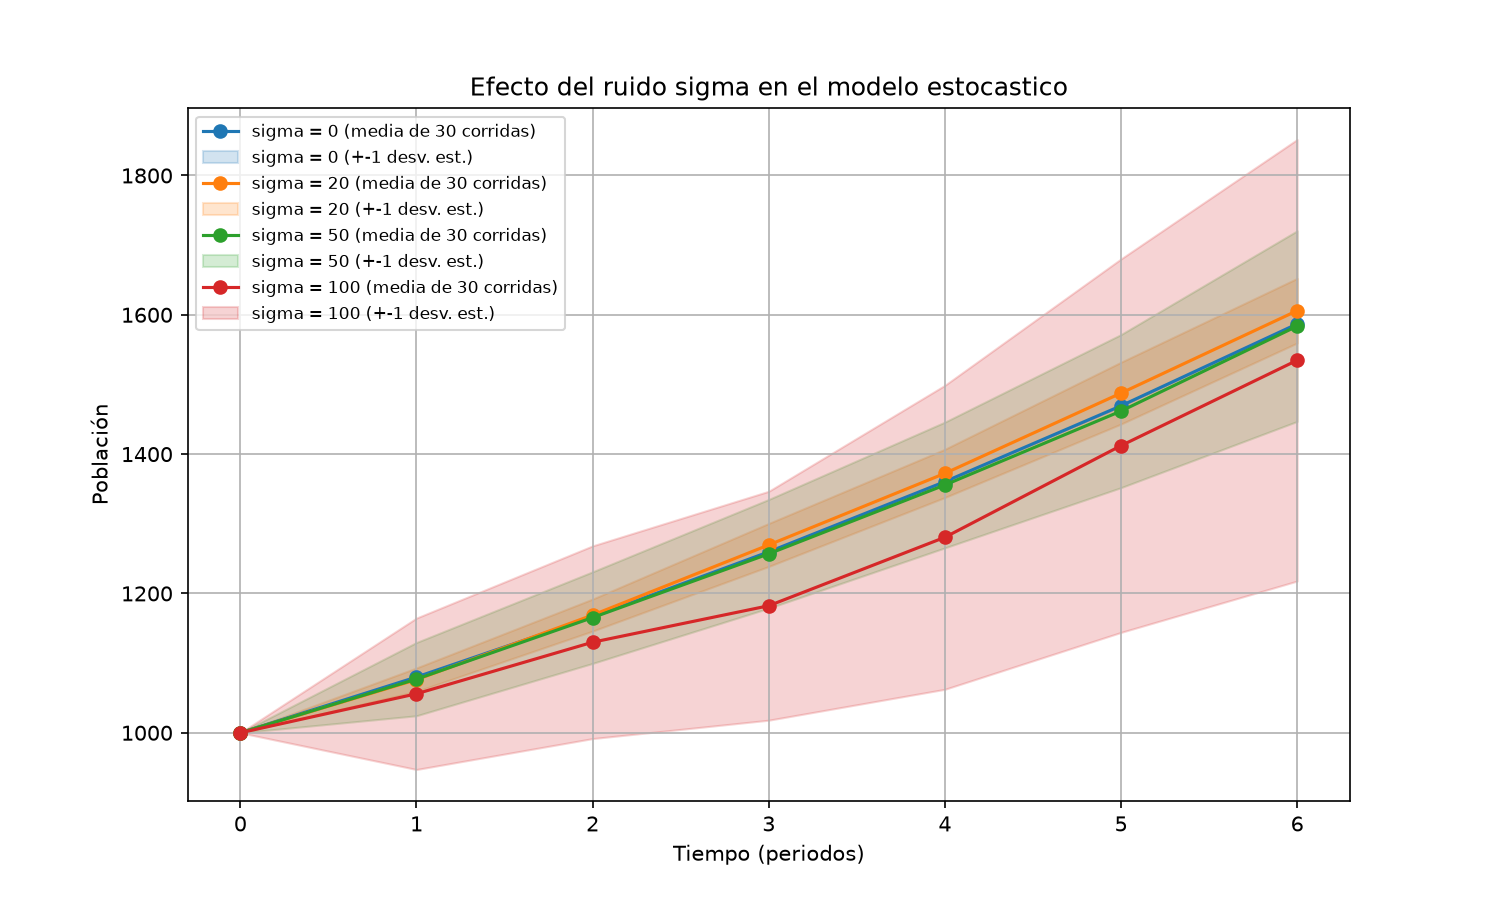
\includegraphics[width=0.92\textwidth]{efecto_sigma.png}
\caption{Efecto del nivel de ruido $\sigma$ en el modelo estoc\'astico (media de $30$
corridas y banda $\pm 1$ desviaci\'on est\'andar).}
\label{fig:sigma}
\end{figure}

Al aumentar $\sigma$ la media se mantiene cercana a la trayectoria determinista, pero la
banda de dispersi\'on se ensancha y crece la proporci\'on de trayectorias que tocan el l\'imite
inferior $0$ por efecto del truncamiento \eqref{eq:truncamiento}.

\subsection{Efecto del paso de integraci\'on ($\Delta t$)}

La figura \ref{fig:dt} compara la soluci\'on de Euler con la exponencial exacta para
distintos pasos. El error decrece al reducir $\Delta t$, confirmando el orden de
convergencia del m\'etodo.

\begin{figure}[htbp]
\centering
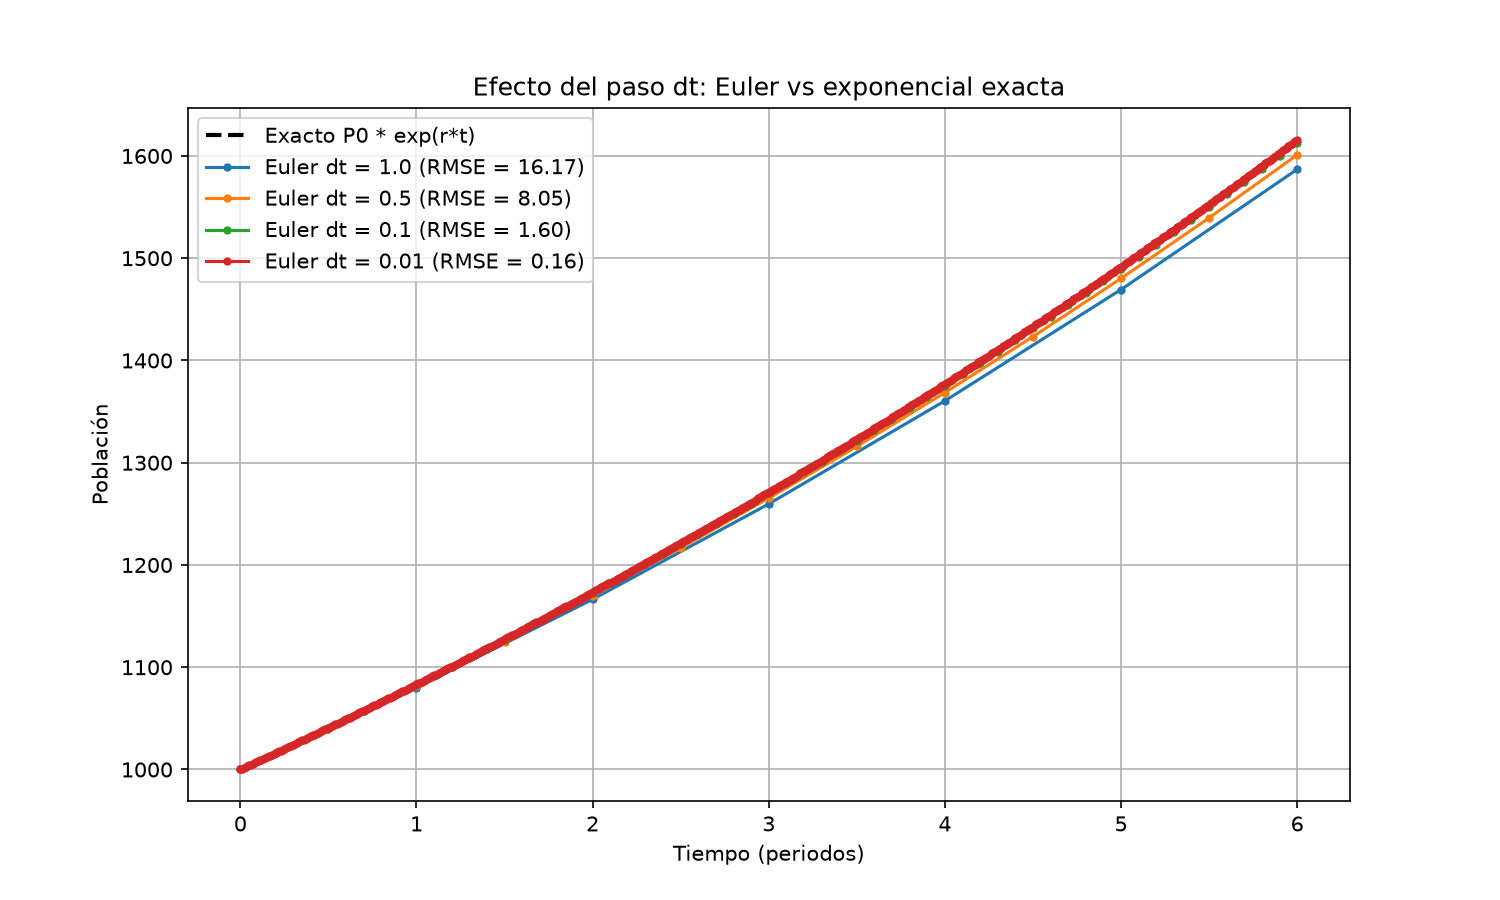
\includegraphics[width=0.92\textwidth]{efecto_dt.png}
\caption{Efecto del paso $\Delta t$: soluci\'on de Euler frente a la exponencial exacta.}
\label{fig:dt}
\end{figure}

\section{Interpretaci\'on Matem\'atica del Comportamiento}

\begin{itemize}[leftmargin=*]
  \item \textbf{Influencia de $r$.} La tasa $r$ gobierna el \emph{tipo} de soluci\'on, no su
        escala. Si $r>0$ el crecimiento es exponencial, pues el incremento $rP$ crece a su
        vez con $P$ (realimentaci\'on positiva); si $r=0$ el sistema permanece en el
        equilibrio $P_0$; si $r<0$ la poblaci\'on decae exponencialmente hacia $0$ de forma
        asint\'otica, sin alcanzarlo en tiempo finito. Cuantitativamente, pasar de
        $r = 0{,}08$ a $r = 0{,}1318$ elev\'o la poblaci\'on final del modelo discreto de
        $1586{,}87$ a $2101{,}57$ y redujo el RMSE de $265{,}29$ a $29{,}61$.
  \item \textbf{Variabilidad frente a tendencia.} El par\'ametro $\sigma$ no altera la
        tendencia del sistema, solo su dispersi\'on: controla el ancho de la distribuci\'on
        de trayectorias alrededor de la curva determinista. El modelo estoc\'astico es, por
        tanto, el \'unico que describe la incertidumbre del sistema; los otros tres
        describen su comportamiento medio.
  \item \textbf{Discreto frente a continuo.} El modelo discreto produce una
        \emph{sucesi\'on} exacta $P_k = P_0(1+r)^k$, mientras el continuo produce la
        \emph{funci\'on} $P(t) = P_0e^{rt}$. Ambos se relacionan a trav\'es del factor
        $(1+r)$ frente a $e^{r}$: son la misma din\'amica descrita con distinta
        discretizaci\'on del tiempo. Euler formaliza ese puente con el factor
        $(1+r\Delta t)$: para $\Delta t = 1$ el m\'etodo coincide con el modelo discreto y
        para $\Delta t \to 0$ converge a la soluci\'on exacta.
  \item \textbf{Naturaleza secuencial de la simulaci\'on.} Los cuatro modelos son
        \emph{recursivos}: cada valor depende del anterior, por lo que el error num\'erico
        (en Euler) y el ruido (en el estoc\'astico) se acumulan a lo largo de los
        per\'iodos. Esto explica por qu\'e la discrepancia entre Euler y la soluci\'on
        exacta crece con el tiempo y por qu\'e la banda de dispersi\'on del modelo
        estoc\'astico se abre progresivamente.
  \item \textbf{Validaci\'on contra datos.} El RMSE permite decidir cu\'al de los cuatro
        paradigmas representa mejor el sistema observado. El resultado
        (RMSE $= 29{,}61$ para el modelo discreto con la tasa estimada) indica que el
        mecanismo subyacente de los datos es multiplicativo por per\'iodo, es decir,
        un proceso discreto y no continuo.
\end{itemize}

\section{Preguntas de Control}

\begin{enumerate}[leftmargin=*]

  \item \textbf{¿Qu\'e representa el arreglo de entrada?}

  Representa la serie de poblaci\'on observada del sistema en siete per\'iodos
  consecutivos: $\left[1000, 1100, 1250, 1400, 1600, 1850, 2100\right]$. No es un
  par\'ametro del modelo, sino la evidencia emp\'irica contra la cual se contrasta la
  simulaci\'on. Cumple tres funciones: fija la condici\'on inicial ($P_0 = 1000$),
  determina el horizonte de simulaci\'on ($6$ per\'iodos) y sirve de referencia de
  validaci\'on para calcular el error de cada modelo.

  \item \textbf{¿Cu\'al es la diferencia entre un modelo determin\'istico y uno
  estoc\'astico?}

  El determin\'istico produce siempre la misma salida para las mismas entradas: el
  resultado queda un\'ivocamente determinado por $P_0$, $r$ y $t$, sin ninguna componente
  aleatoria. El estoc\'astico incorpora al menos una variable aleatoria
  ($\varepsilon_k \sim \mathcal{N}(0,\sigma^{2})$), de modo que cada repetici\'on arroja una
  trayectoria distinta; su salida no es un valor \'unico sino una distribuci\'on de
  resultados que se describe con media y varianza \cite{lawkelton2015,banks2010}. En
  t\'erminos de la simulaci\'on, el primero es reproducible por definici\'on y el segundo
  solo lo es si se fija la semilla del generador aleatorio.

  \item \textbf{¿Qu\'e efecto produce modificar la tasa ($r$)?}

  Cambia el tipo y la rapidez del comportamiento. Si $r>0$ hay crecimiento exponencial, y
  tanto m\'as r\'apido cuanto mayor sea $r$; si $r = 0$ el sistema permanece constante en
  $P_0$; si $r<0$ la poblaci\'on decrece exponencialmente. El efecto es multiplicativo y se
  acumula: pasar de $r = 0{,}08$ a $r = 0{,}1318$ elev\'o el valor final del modelo
  discreto de $1586{,}87$ a $2101{,}57$ y redujo el RMSE de $265{,}29$ a $29{,}61$.

  \item \textbf{¿Qu\'e representa el par\'ametro ($\sigma$)?}

  Es la desviaci\'on est\'andar del ruido aditivo normal de media cero que se suma en cada
  per\'iodo. Representa el \textbf{nivel de variabilidad o incertidumbre} del sistema: no
  modifica la tendencia, sino la dispersi\'on de las trayectorias alrededor de ella. El caso
  l\'imite $\sigma = 0$ degenera el modelo estoc\'astico en el modelo discreto
  determin\'istico.

  \item \textbf{¿Qu\'e ocurre cuando aumenta el nivel de ruido?}

  La media de las trayectorias se mantiene cercana a la curva determinista, pero la banda
  $\pm 1$ desviaci\'on est\'andar se ensancha de forma progresiva, de modo que las
  trayectorias individuales se vuelven cada vez m\'as impredecibles. Adem\'as, al crecer
  $\sigma$ aumenta la probabilidad de que el ruido empuje la poblaci\'on por debajo de cero
  y active el truncamiento \eqref{eq:truncamiento}; como ese l\'imite es absorbente hacia
  abajo, se introduce un sesgo que hace que la media quede ligeramente por debajo de la
  trayectoria determinista.

  \item \textbf{¿Cu\'al es la diferencia entre los modelos discreto y continuo?}

  El discreto solo est\'a definido en instantes separados (per\'iodos enteros) y genera la
  sucesi\'on $P_k = P_0(1+r)^{k}$, que es exacta para esa formulaci\'on. El continuo est\'a
  definido para todo $t$ real y genera la funci\'on $P(t) = P_0e^{rt}$; al resolverse
  num\'ericamente con Euler, introduce un error de truncamiento que el modelo discreto no
  tiene. La diferencia conceptual es el dominio de definici\'on del tiempo; la diferencia
  pr\'actica es que el modelo discreto es un m\'etodo de un paso con $\Delta t = 1$, mientras
  el continuo permite refinar la resoluci\'on temporal.

  \item \textbf{¿Qu\'e funci\'on cumple ($\Delta t$)?}

  Es el tamaño del paso de integraci\'on num\'erica del m\'etodo de Euler y controla dos
  aspectos: la resoluci\'on temporal de la soluci\'on aproximada y el error de
  truncamiento, que es de primer orden $O(\Delta t)$ \cite{burden2011}. Reducir $\Delta t$
  acerca la soluci\'on num\'erica a la exponencial exacta, como se observa en la
  figura \ref{fig:dt}. El caso $\Delta t = 1$ hace que Euler coincida exactamente con el
  modelo discreto, lo que muestra que ambos paradigmas comparten el mismo c\'alculo.

  \item \textbf{¿Por qu\'e es importante visualizar los resultados mediante gr\'aficas?}

  Porque una tabla solo muestra valores puntuales y no revela la \emph{forma} del
  fen\'omeno (exponencial, lineal o con saturaci\'on), ni permite distinguir a simple vista
  una trayectoria con ruido de una determinista, ni apreciar el error de un m\'etodo
  num\'erico. La gr\'afica expone de manera inmediata la tendencia, la dispersi\'on y el
  error, y permite comparar los cuatro paradigmas de un solo vistazo; en esta pr\'actica
  es lo que hizo evidente que la serie observada crec\'ia m\'as r\'apido que el modelo con
  $r = 0{,}08$.

  \item \textbf{¿Qu\'e modelo presenta comportamiento aleatorio?}

  \'Unicamente el modelo estoc\'astico, por la presencia del t\'ermino aleatorio
  $\varepsilon_k \sim \mathcal{N}(0,\sigma^{2})$ en la ecuaci\'on \eqref{eq:estocastico}.
  Los otros tres son determin\'isticos y, con la misma condici\'on inicial y los mismos
  par\'ametros, producen siempre exactamente la misma trayectoria.

  \item \textbf{¿C\'omo cambia la simulaci\'on cuando se introduce un nuevo arreglo de
  datos?}

  Cambian autom\'aticamente tres elementos: la poblaci\'on inicial pasa a ser el primer
  valor del nuevo arreglo, el horizonte de simulaci\'on pasa a ser el n\'umero de elementos
  menos uno, y los valores de referencia del RMSE se actualizan. En cambio, $r$ y $\sigma$
  \textbf{no} se recalculan solos, porque son par\'ametros de entrada del modelo y no
  propiedades de los datos; si se quiere que el modelo se reajuste a la nueva serie se debe
  activar la estimaci\'on autom\'atica de $r$ incluida en el programa
  (\texttt{-{}-ajustar-r}). Esto se verific\'o ejecutando la simulaci\'on con distintos
  valores de $r$, con $r$ negativa y con la tasa estimada desde los datos.

\end{enumerate}

\section{Conclusiones}

\begin{itemize}[leftmargin=*]
  \item Se implementaron correctamente los cuatro paradigmas solicitados
        (determin\'istico, discreto, estoc\'astico y continuo por Euler) sobre un mismo
        sistema de crecimiento poblacional, lo que permiti\'o compararlos sobre una base
        com\'un y cuantificar sus diferencias mediante el RMSE.

  \item Se identific\'o que la tasa $r$ es el par\'ametro que determina el tipo de
        comportamiento del sistema (crecimiento, equilibrio o decrecimiento) y que su
        valor condiciona fuertemente la calidad del ajuste. Estimar $r$ desde los datos
        ($\hat{r} = 0{,}1318$) redujo el RMSE del modelo discreto de $265{,}29$ a
        $29{,}61$, convirti\'endolo en el paradigma que mejor representa la serie
        observada.

  \item Se comprob\'o que el par\'ametro $\sigma$ controla exclusivamente la
        aleatoriedad del sistema, sin alterar su tendencia, y que $\Delta t$ controla el
        error de la aproximaci\'on num\'erica del modelo continuo; el caso
        $\Delta t = 1$ demuestra que el modelo discreto y el continuo son la misma
        din\'amica vista con distinta resoluci\'on temporal.

  \item La visualizaci\'on gr\'afica result\'o indispensable: fue la que evidenci\'o que la
        serie observada crec\'ia a un ritmo distinto al del par\'ametro inicial de la
        gu\'ia y permiti\'o detectar el sesgo que introduce el truncamiento de la
        poblaci\'on en el modelo estoc\'astico con ruido elevado.
\end{itemize}

\newpage

\section{Declaraci\'on de Uso de Inteligencia Artificial}

En cumplimiento de los principios de solidaridad, transparencia, responsabilidad y
honestidad establecidos en el resultado de aprendizaje R1, se declara lo siguiente:

\begin{enumerate}[leftmargin=*]
  \item \textbf{Porcentaje de uso.} Se emplearon herramientas de inteligencia artificial
        como apoyo acotado, estimado en \textbf{no m\'as del 20\%} del trabajo total de
        la pr\'actica.

  \item \textbf{El razonamiento del estudiante no fue reemplazado.} La comprensi\'on del
        problema, la selecci\'on y justificaci\'on de los cuatro modelos, la
        interpretaci\'on matem\'atica del comportamiento, la estimaci\'on de la tasa $r$ y
        las respuestas a las preguntas de control fueron razonadas, revisadas y validadas
        por el estudiante.

  \item \textbf{Alcance del apoyo recibido.} El uso de la IA se limit\'o a tareas
        auxiliares: la traducci\'on del pseudoc\'odigo de la gu\'ia a c\'odigo Python, el
        diseño y formato de las gr\'aficas, y la revisi\'on de estilo y redacci\'on de la
        documentaci\'on. Ninguna decisi\'on metodol\'ogica se deleg\'o a la herramienta.

  \item \textbf{Verificaci\'on de resultados.} Todos los valores presentados en este
        reporte provienen de la ejecuci\'on reproducible del programa desarrollado
        (\texttt{python -m views.main}), con semilla fija para el modelo estoc\'astico. El
        estudiante ejecut\'o, comprob\'o y comprendi\'o cada resultado antes de incluirlo.

  \item \textbf{Responsabilidad.} El estudiante asume la responsabilidad total sobre el
        contenido, la exactitud, la originalidad y las conclusiones del trabajo entregado.
\end{enumerate}

\bibliographystyle{IEEEtran}
\bibliography{referencias}

\end{document}
